\chapter{Обзор концепций, алгоритмов и программных средств по теме исследования}\label{ch:ch1}

\section{Визуальные языки программирования}\label{sec:ch1/sec1}

Для объяснения принципа работы программы, программисты часто используют
графические модели, вроде блок-схем и диаграмм UML. Ввиду удобства графических
обозначений, возникает интерес в использовании подобных нотаций для
написания компьютерных программ. Такую концепцию создания программного обеспечения
реализуют визуальные языки программирования.

\textbf{Визуальный язык программирования} --- язык программирования, 
который позволяет пользователю создавать программы, манипулируя элементами
программы графически, а не задавая их в виде текста \cite{maturityofvpl}.

Главное назначение визуальных языков программирования --- сделать 
программирование более доступным людей без опыта с ним,
улучшить пользовательских опыт программиста на трёх уровнях \cite{agentsheetsmovingbeyondsyntax}:

\begin{itemize}
    \item \textbf{на уровне синтаксиса} --- элементы визуальных языков вместо текста 
    представлены строго в виде пиктограмм, блоков, диаграмм, что исключает возможность
    наличия в программе синтаксических ошибок.
    \item \textbf{на уровне семантики} --- графическое представление объектов
    языка позволяет наглядно показать назначение программных примитивов, и тем
    самым сократить время обучения языку.
    \item \textbf{на прикладном уровне} --- многие визуальные языки позволяют
    перевести программу в определенное состояние с целью исследования, как поведет
    себя программа в данном состоянии.
\end{itemize}

\section{Типы визуальных языков программирования}\label{sec:ch1/sec2}

\subsection{Блочные языки}\label{sech:ch1/sec2/sub1}

Блочные языки позволяют составлять программы из блоков-инструкций.
Управляющие конструкции блочных языков в целом копируют классические языки,
но графические подсказки помогают понять, как комбинировать базовые элементы,
такие как переменные, процедуры и операторы. В блоках используются текстовые 
обозначения для задания имен и значений переменных.

В сравнении с другими графическими языками, программы на блочных языках
близки к исходному коду на императивных языках, однако использование
визуальных блоков позволяет избежать ошибок за счет ограничений языка.

На рисунке~\ref{fig:blockly} приведен пример программы, три раза выводящей
на экран сообщение <<Hello World!>>, на блочном языке Blocky \cite{blocklysite}.
\begin{figure}[ht]
	\centering
	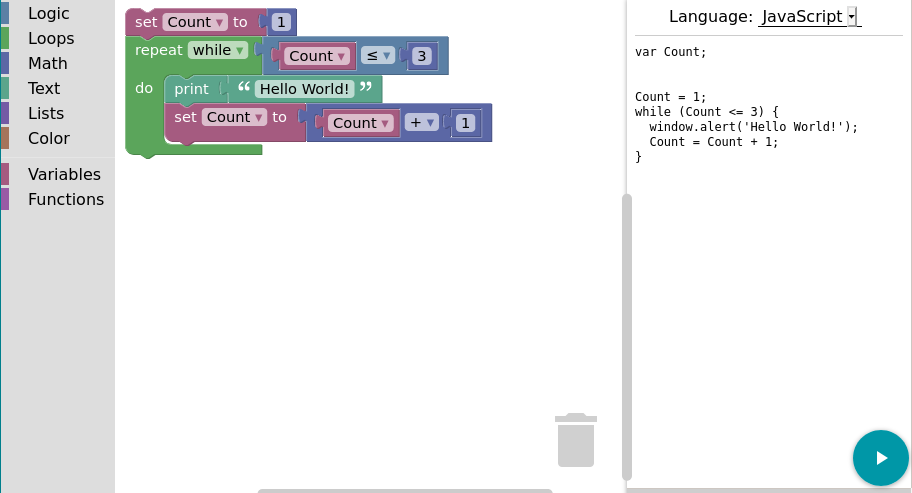
\includegraphics [scale=0.65] {blockly}
	\caption{Пример программы на блочном языке}
	\label{fig:blockly}
\end{figure}

\FloatBarrier

\subsection{Языки, основанные на блок-схемах}\label{sech:ch1/sec2/sub2}

Существуют визуальные языки, использующие представление, близкое к
блок-схемам, для описания главного потока управления программы. Программы
на таких языках представлены набором блоков, соединенных между собой линиями, 
задающими последовательность исполнения инструкций.

Простая визуальная грамматика и упор на исполнение программ делают такие
языки легкими в освоении, однако программы на таких языках быстро
разрастаются и становятся трудночитаемыми.

На рисунке~\ref{fig:flowgorithm} приведен пример программы 
на языке Flowgorithm \cite{flowgorithm}, основанном на блок-схемах.
\begin{figure}[ht]
	\centering
	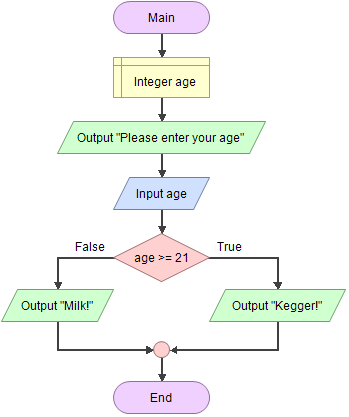
\includegraphics [scale=0.65] {flowgorithm}
	\caption{Пример программы на языке, основанном на блок-схемах}
	\label{fig:flowgorithm}
\end{figure}

\FloatBarrier

\subsection{Языки программирования потоков данных}\label{sech:ch1/sec2/sub3}

Наиболее часто в профессиональных программных комплексах используются
визуальные языки программирования потоков данных. Как правило, такие
языки ориентированы на специалистов, не использующих текстовые языки
программирования в своей повседневной работе.

В программировании потока данных блок представляют функции, связанные
с собой потоком данных, от входа к выходу. Создавая связи между
точкой выхода одного блока и точкой входа другого блока, программист
задает поток выполнения программы через поток данных.

Множество процессов реальной жизни может быть промоделировано с помощью
потоков данных, поэтому визуальные языки подобного рода часто 
используются как встраиваемые языки предметной области в сложных
конфигурируемых программных продуктах: системах потоковой обработки
информации, игровых движках, пакетах компьютерной графики.

На рисунке~\ref{fig:blueprint} приведен пример программы 
на языке программирования потоков данных Blueprint \cite{blueprint}, 
используемого для создания пользовательских сценариев в игровом движке
Unreal Engine 4.
\begin{figure}[ht]
	\centering
	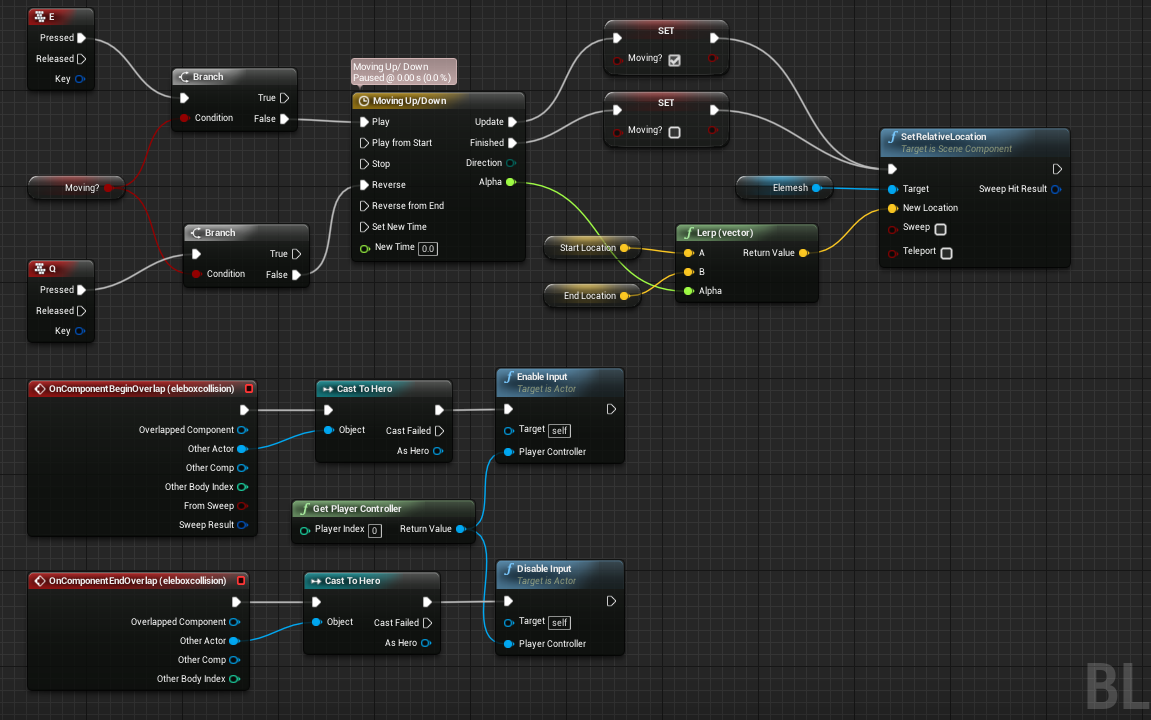
\includegraphics [scale=0.45] {blueprint}
	\caption{Пример программы на языке программирования потоков данных}
	\label{fig:blueprint}
\end{figure}

\FloatBarrier

\section{Функциональное программирование}\label{sec:ch1/sec3}

Большинство языков программирования основываются на идее, что описываемые
программы подразумевают в своей работе изменение значений набора переменных.
Такой набор переменных называют \textit{состоянием} программы.

За изменение состояния программы отвечают операторы присваивания, а составные
операторы, такие как \textbf{if} и \textbf{while}, позволяют выполнять участки программы
в зависимости от условия или циклически.

Готовая программа представляет собой \textit{набор инструкций}, изменяющих
состояние программы и опирающихся на него. Такой подход к описанию программ 
известен как \textit{императивное программирование}.

В противовес императивному программированию предлагается подход к описанию
и выполнению программ, в общем виде не опирающийся на состояние. Такой подход
имеет название \textit{<<функциональное программирование>>}.

\textbf{Функциональное программирование} --- это стиль или парадигма
программирования, в которой программа представляет собой выражение, а
выполнение программы --- процесс вычисления этого выражения \cite{harrison97}. % страница 1

Под выражением здесь понимается программная сущность, которая
может быть вычислена для получения ее значения \cite[с.~26]{sicp}. % страница 26 на русском

Выражениями являются как значения простых типов (такие как целые числа),
так и комбинации выражений, в том числе --- применение функции к аргументам.

Процесс применения функции к аргументом имеет название \textit{аппликации}, языки,
основывающиеся на этой концепции, имеют название \textit{аппликативных}. Термин
\textit{аппликативное программирование} часто используется как синоним к функциональному
программированию.

Под функцией в функциональном программировании подразумевается математическое определение функции, 
то есть --- правило $f$, позволяющее для каждого элемента $a$ множества $A$ найти соответствующий 
ему элемент $f(a)$ множества $B$ \cite[с.~12]{algrebrakirkinskii}: % страница 12

\begin{equation}
    \label{eq:function_equation}
    f : A \rightarrow B.
\end{equation}

В общем случае, исходя из определения, функциональное программирование 
не подразумевает наличия в программе переменных, следовательно, и состояния 
программы.

Связанные с функциональным программированием концепции и понятия рассмотрены
далее в разделе.

\subsection{Система функционального программирования по Бэкусу}\label{sec:ch1/sec3/subsec1}

На вручении премии Тьюринга в 1977 году, исследователь языков программирования Джон Бэкус
выступил с лекцией <<Можно ли освободить программирование от стиля фон Неймана? Функциональный
стиль и соответствующая алгебра программ>> (оригинальное название -- <<Can 
Programming Be Liberated from the von Neumann Stye? A Functional Style and
Its Algebra of Programs>>) \cite{backus77}. В докладе Бэкус представил функциональные языки
как альтернативу традиционному императивному программированию, описал
неформальную и формальную системы функционального программирования, ввел
алгебру функциональных программ для этих систем.

Неформальное описание представляет систему функционального программирования
в упрощенном виде, удобном для знакомства с структурами подобного рода.

Система функционального программирования включает \cite[с.~620]{backus77}:
\begin{enumerate}
    \item множество \textit{объектов} $O$,
    \item множество \textit{функций} $F$, отображающих объекты в объекты;
    \item операцию \textit{применения};
    \item множество \textit{функциональных форм} \textit{\textbf{F}}, 
    используемых для комбинирования существующих функций или объектов,
    для задания новых функций из $F$;
    \item множество \textit{описаний} $D$, определяющих функции в $F$ и присваивающих им имя.
\end{enumerate}

Ниже следует описание каждой сущности.

\textbf{Объекты, О}. \textit{Объект $x$} является либо \textit{атомом},
либо последовательностью $<x_1, \dots, x_n>$, элементы которой являются
либо объектами, либо специальным атомом, обозначающим неопределенное значение.
Исходя из определения объекта, набор атомов $A$ определяет множество
объектов. Элементы множества атомов $A$ определяются непустыми строками,
состоящими из любых кодируемых символов, не задействованных в нотации системы.
Символом {\O} обозначается пустая последовательность, также являющаяся
атомом.

На последовательности накладывается ограничение --- если последовательность $x$
содержит неопределенное значение, то $x$ им и является. Следуя из ограничения,
не существует ни одной последовательности, содержащей неопределенное значение.

\textbf{Применение}. Система функционального программирования имеет одну
операцию применения, также называемую \textit{аппликацией}. Пусть $f$ ---
функция, а $x$ --- объект, тогда $f:x$ --- аппликация, результатом которой
является объект, получаемый после применения $f$ (функции-оператора) 
к $x$ (операнду).

\textbf{Функции}. Функции в $F$ отображают объекты в объекты, и для каждой
функции $f$ применение к неопределенному значению дает неопределенное значение.
Каждая функция в $F$ является либо \textit{примитивной}, то есть, задаваемой
в системе, либо \textit{описываемой} пользователем, либо \textit{функциональной формой}.

Если вычисление $f:x$ завершается и дает неопределенное значение, функция
$f$ считается \textit{неопределенной} в $x$. Иначе $f$ называют
\textit{незавершаемой} в $x$.

\textbf{Функциональные формы, F}. Функциональной формой называется выражение,
обозначающее функцию, которая зависит от функций или объектов, называемых
\textit{параметрами} выражения. 

Примером функциональной формы является композиция функций $f$ и $g$, 
определяемая как функция $f \circ g$, такая, что для любого объекта $x$:
$(f \circ g) : x = f : (g : x)$.

Функциональными формами определяются конструкции, которые нельзя выразить
через другие элементы системы функционального программирования, такие как
условные выражения.

\textbf{Определения}. Определением в системе функционального программирования
называется выражение вида \textbf{Def} $l$ = $r$, где левая
часть $l$ --- неиспользованный символ функции, а правая часть $r$ ---
функциональная форма, возможно, зависящая от $l$. Оно выражает тот факт, что
символ $l$ обозначает функцию, заданную через $r$. Для применения определенного
символа, следует заменить его на правую часть его определения.
Множество определений $D$ считается \textit{правильным}, если никакие
левые части в нем не совпадают.

Для понимания семантики системы функционального программирования, нужно знать, как
вычислить $f:x$ для произвольной функции $f$ и произвольного объекта $x$
в системе с четверкой $<A, P, F, D>$, где $A$ --- множество атомов,
$P$ --- множество примитивных функций, \textbf{F} --- множество функциональных
форм, $D$ --- правильное множество определений.

$f$ может определяться как:
\begin{itemize}
    \item примитивная функция;
    \item функциональная форма;
    \item определение \textbf{Def} $f \equiv r$;
    \item что-либо, отличное от вышеперечисленного.
\end{itemize}

Если $f$ является примитивной функцией, то существует ее определение и известен
порядок ее вычисления. Если $f$ --- функциональная форма, то определение
формы включает правило вычисления $f:x$ в терминах параметров формы, и может
быть сведено к примитивным функциям, другим функциональным формам, определениям
в дальнейшем. Если $f$ определена как \textbf{Def} $f \equiv r$, то
$f:x$ находится подстановкой $f:x, f \equiv r \Rightarrow r:x$. При ином $f$
и в случае незавершения вычислений при некоторых $f$ и $x$, $f:x$ является
неопределенным значением.

\subsection{Чистые функции}\label{sec:ch1/sec3/subsec2}

По определению, функция отображает каждый элемент из области определения
в единственный элемент из ее области значений.
Следовательно, нет неоднозначности в том, в какой элемент
из области значений переводится заданный элемент из области
определения функции. Иными словами, для заданных входных данных
функция всегда возвращает одинаковый результат. Данное свойство
называют \textbf{детерминированностью}, а функции, ему удовлетворяющие, ---
\textbf{детерминированными} \cite[с.~12]{fp93}.

Другим следствием из математического понятия функции, является тот факт,
что любое выражение определяет единственное значение, которое нельзя
изменить путем его вычисления --- вычисление изменяет форму выражения, но не
величину, например: $f(x) = x, f(10) \equiv 10$. Данное свойство имеет
название \textbf{<<ссылочная прозрачность>>} \cite{sorengardsestoftreftransp}.
В компьютерной программе это свойство поддерживается, если совместное
использование выражения также исключает изменение его значения.
Нетрудно заметить, что переменные в императивных языках не являются
ссылочно-прозрачными, так как могут быть изменены операцией присваивания,
и использующие их функции, при одних входных данных могут возвращать
разный результат, тем самым нарушая свойство детерминированности.
Изменения в программе, которые могут нарушать детерминированность некоторых
функций, называют \textbf{побочными эффектами} \cite[с.~17]{fp93}.
Другим примером побочных эффектов является организация ввода-вывода:
возможно чтение данных из файла, ранее отредактированного другим пользователем;
запись данных подразумевает изменение состояния файловой системы и накопителя данных.

Функция называется \textbf{чистой}, если:

\begin{itemize}
    \item является детерминированной;
    \item не имеет побочных эффектов (не ссылается на данные, 
     значения которых могут измениться в процессе работы программы
     и не производит таких изменений) \cite{purefunctions}.
\end{itemize}

Программы, состоящие из чистых функций, могут быть распараллелены
компилятором, так как в данном случае отстутствуют зависимости по данным
и необходимость синхронизации \cite[182]{staroletovfunlang}.

\subsection{Функции первого класса и функции высшего порядка}\label{sec:ch1/sec3/subsec3}

В языках программирования объектами \textit{первого класса} называют такие
программные сущности, которые можно:

\begin{itemize}
    \item называть с помощью переменных;
    \item передавать в функции в качестве параметров;
    \item получать из функций в виде результата;
    \item включать в структуры данных \cite[с.~87]{sicp}.
\end{itemize}

Если в языке программирования для функций выполнены вышеперечисленные условия,
им дается название \textbf{функций первого класса}.

\textbf{Функция высшего порядка} --- функция, которая может использовать в
качестве аргумента другую функцию или результатом выполнения которой является
некоторая функция \cite[с.~56]{fp93}.

С помощью функций высшего порядка можно зафиксировать часть параметров $n$-арной
функции, получив тем самым другую функцию меньшей арности.
Такая операция имеет название \textbf{частичного применения}
(англ. --- partial application) \cite{partialapplication}. 
Частичное применение функций играет особую роль в реализации ленивой стратегии вычислений.

\subsection{Строгие и ленивые вычисления}\label{sec:ch1/sec3/subsec4}

В большинстве языков программирования при вызове функции сначала вычисляются
ее аргументы, которые затем передаются в функцию. Такой подход
--- <<вычисление аргументов, затем применение функции>> ---
имеет название \textbf{аппликативного порядка вычисления}, а механизм вызова,
реализующий такой порядок называется \textbf{вызовом по значению}. Класс
семантических правил, требующих вычисления аргументов до применения к ним
функции называют \textbf{строгими вычислительными стратегиями} \cite[с.~71]{fp93}.

Альтернативой такому подходу является передача в функцию выражений-аргументов
в невычисленном виде, которые будут вычислены при необходимости в теле
функции. Модель <<полная подстановка, потом сведение к значениям>> называют
\textbf{нормальным порядком вычисления}, реализующий ее метод вызова функций
--- \textbf{вызовом по необходимости}. В противовес строгим стратегиям,
такие подходы имеют название \textbf{нестрогих} или \textbf{ленивых вычислительных
стратегий} \cite[с.~32]{sicp}\cite[с.~370]{sicp}.

Основная идея реализации ленивых вычислений заключается в преобразовании
невычисленных аргументов в специальные объекты, называемые \textbf{задумками}
(англ. --- \textit{thunk}). Задумки содержат информацию, необходимую для
вычисления значения аргумента --- выражение-аргумент и окружение, в котором
вычисляется вызов функции. Процесс вычисления задумки называется
\textbf{форсированием задумки} (англ. --- \textit{forcing a thunk}) и происходит, когда требуется ее значение \cite[с.~372]{sicp}.

При реализации интерпретаторов и компиляторов, поддерживающих ленивые вычисления,
удобно реализовывать задумки с использованием частичного применения функций.
В таком случае вместо вычисления значения будем иметь функцию-задумку,
при вычислении (форсировании) которой получим требуемый аргумент \cite[с.~375]{sicp}.

Обе модели вычислений имеют свои преимущества и недостатки: для строгих
вычислений просто реализовать эффективную реализацию путем накопления по
дереву выражений \cite[с.~29]{sicp}, но возможны избыточные вычисления,
когда значение аргумента не требуется функции; в случае ленивых вычислений
неиспользуемые аргументы не вызовут лишних затрат на вычисления, однако
повлияют создание задумок и передача их внутрь функции.

\subsection{Рекурсия}\label{sec:ch1/sec3/subsec5}

Для организации повторяющихся вычислений в функциональных языках используется
рекурсия. Рекурсивные функции вызывают сами себя, пока не достигнут терминальной
ветви. Рекурсия требует стек вызовов, размер которого растет линейно к
глубине рекурсии, рекурсивные функции с большой глубиной могут вызвать
переполнение стека, что ставит рекурсию в проигрышное положение по сравнению
с классическими циклами. Однако существует класс рекурсивных функций,
процесс вычисления которых может быть сведен к императивному циклу. Оптимизация
таких функций и других шаблонов рекурсии имеет особое значение в реализации
функциональных языков программирования и \textit{рассматривается далее в работе}.

\section{Elm-архитектура}\label{sec:ch1/sec4}

Функциональные программы представляют процесс вычисления чистых функций,
не подразумевают наличие изменяемых данных и состояния программы, поэтому
использование классических архитектурных шаблонов, таких как 
Model-View-Controller --- (MVC, <<Модель-Представление-Контроллер>>) 
не представляется возможным.

В чистом функциональном языке программирования Elm представлен одноименный
паттерн, позволяющий строить интерактивные программы, такие как веб-приложения и игры,
с использованием функциональных языков \cite{elmarchitecture}.

Шаблон также имеет название Model-View-Update, по именам его компонентов --- модели, представления
и функции обновления.

Структурно Elm-архитектуру можно представить следующим образом: 

\begin{figure}[ht]
	\centering
	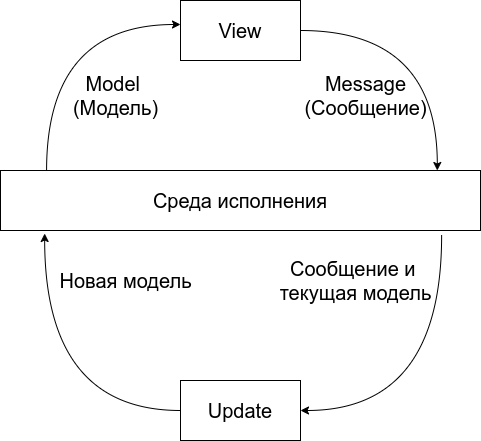
\includegraphics [scale=0.45] {tea}
	\caption{Структурная схема Elm-архитектуры}
	\label{fig:elmarch}
\end{figure}

\FloatBarrier

На рисунке \ref{fig:elmarch}:

\begin{itemize}
    \item модель (англ. --- model) --- описание данных программы. Просто тип данных --- примитивный или составной. Модель представляет состояние приложения;
    \item представление (англ. --- view) --- отображение данных, представляется как чистая функция. Принимает модель из источника, строит и отображает пользовательский интерфейс.
    Если с документом совершено какое-либо пользовательское действие (пользователь нажал на кнопку, набрал текст в поле ввода), порождает сообщение, которое отправится в Update;
    \item сообщения --- значения, используемые для передачи информации из одной части системы в другие;
    \item функция обновления (англ. --- update) --- функция, преобразующая текущую модель по полученному сообщению;
    \item среда исполнения --- программное окружение, распределяющее информацию между компонентами системы.
\end{itemize}

Цикл жизни программы, построенной с использованием Elm-архитектуры:

\begin{enumerate}
    \item на основе модели в \textit{View} отрисовывается интерфейс;
    \item при пользовательском действии в \textit{Update} посылается сообщение;
    \item в функции \textit{Update} обрабатывается текущая модель данных программы и посланное сообщение, функция возвращает новую модель, инициируется перерисовка \textit{View} \cite{elminaction}.
\end{enumerate}

\FloatBarrier

\section{Компиляторы}\label{sec:ch1/sec5}

\textbf{Компилятор} --- программа, которая считывает текст программы, написанной
на \textit{исходном} языке, и транслирует его в эквивалентный текст на
\textit{целевом} языке \cite[с.~29]{dragonbook}.

Процесс компиляции представляет собой последовательность фаз (проходов),
преобразующих одно из представлений программы в другое \cite[с.~33]{dragonbook}.

В зависимости от решений при проектировании, количество фаз может варьироваться
от 2 до 70, однако в большинстве современных компиляторов используется
три большие фазы: преобразование текста программы в программное представление,
манипуляции с программным представлением и синтез программы.

\subsection{Структура трёхпроходного компилятора}\label{sec:ch1/sec5/subsec1}

Структурно трёхпроходный компилятор представляется следующим образом:

\begin{figure}[ht]
	\centering
	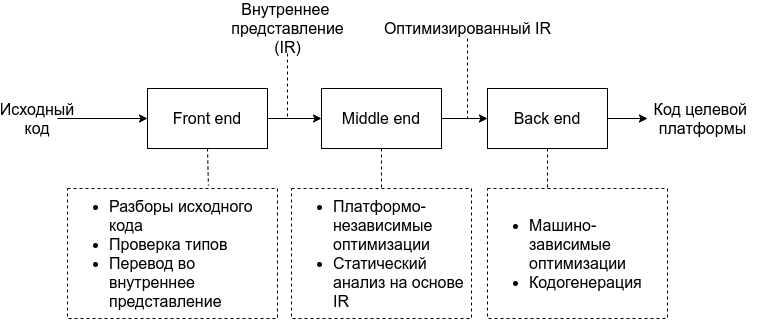
\includegraphics [scale=0.45] {multi-pass}
	\caption{Структурная схема многопроходного компилятора}
	\label{fig:triphasecompiler}
\end{figure}

\FloatBarrier

Исходный код программы разбирается лексическим и синтаксическим анализатором,
проходит проверку на контекстные условия и переводится во внутреннее представление
в блоке, именуемом фронт-эндом компилятора \cite[с.~6]{engineeringacompiler}.

\textbf{Промежуточное представление} (англ. --- intermediate representation) ---
структура данных, используемая внутри компилятора для представления исходного
кода программы \cite[с.~221]{moderncompilerml}.

Полученное во фронт-энде промежуточное представление поступает в блок, именуемый
миддл-эндом, или оптимизатором, в котором изменяется с целью проведения независимых
от платформы оптимизаций. Оптимизированное представление отправляется в бэк-энд компилятора,
в котором происходит синтез программы на целевом языке.

\subsection{Фронт-энд компилятора}\label{sec:ch1/sec5/subsec2}

Первый этап компиляции во фронт-энде называется \textbf{лексическим анализом}.
Лексический анализатор читает поток символов, составляющих текст исходной
программы, и группирует их в \textit{лексемы}. Для каждой лексемы строится
\textit{токен}, содержащий ее значение, поток токенов передается синтаксическому
анализатору \cite[с.~33]{dragonbook}.

\textbf{Синтаксический анализатор} или \textbf{парсер} на основе токенов,
полученных при лексическом анализе, строит древовидное внутреннее представление,
такое как \textit{синтаксическое дерево} \cite[с.~35]{dragonbook}.

С помощью синтаксического дерева \textbf{семантический анализатор} проверяет
исходную программу на семантическую достоверность определению языка. Частью
семантического анализа является \textbf{проверка типов}, то есть согласование
сущностей программы по их типам \cite[с.~37]{dragonbook}.

После проверки семантическим анализатором, на основе синтаксического
дерева строится промежуточное представление программы, используемое другими
блоками компилятора. Синтаксическое дерево также является видом промежуточного
представления, однако используется чаще всего в процессе синтаксического
и семантического анализа; на других этапах отдается предпочтение представлениям,
которые легко генерируются и транслируются в целевой язык \cite[с.~38]{dragonbook}.

\subsection{Виды промежуточных представлений компилятора}\label{sec:ch1/sec5/subsec3}

Промежуточные представления делятся на три категории:

\begin{itemize}
    \item \textit{Графовые} промежуточные представления
    представляют программу в виде графа и выражаются в
    узлах, дугах, деревьях.
    \item \textit{Линейные} промежуточные представления
    напоминают псевдокод для некоторой абстрактной маишны.
    \item \textit{Гибридные} промежуточные представления
    совмещают элементы графовых и линейных представлений,
    и являются попыткой соединить их сильные стороны, избежав
    слабостей. Обычно гибридные представления используют
    линейные части для представления блоков последовательного
    кода, и графы для представления потока управления между
    этими блоками \cite[с.~223]{engineeringacompiler}.
\end{itemize}

\subsection{Графовые промежуточные представления. Граф зависимостей}\label{sec:ch1/sec5/subsec4}

\textbf{Граф зависимостей по данным} --- поток значений из точки, в которой
значение создано, \textit{определения} (англ. --- definition), в точку,
где оно используется, или \textit{использование} (англ. --- use) \cite[с.~232]{engineeringacompiler}.

\begin{figure}[ht]
	\centering
	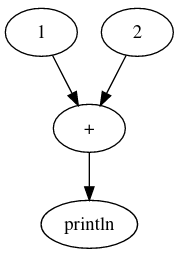
\includegraphics [scale=0.75] {dep_graph}
	\caption{Граф зависимостей по данным для выражения println(1 + 2)}
	\label{fig:depgraph}
\end{figure}

\FloatBarrier

Графы зависимостей по данным часто используются как вспомогательное
промежуточное представление. Они играют центральную роль в планировании
команд в целевой программе, так как позволяют установить порядок вычислений.

Для упорядочения инструкций по графу зависимостей используется алгоритм
топологической сортировки, упорядочивающий граф в линейную последовательность
вершин, такую, что пары вершин, связанных отношением зависимости в нём
идут строго слева направо \cite[с.~643]{engineeringacompiler}.

Простой алгоритм топологической сортировки Тарьяна заключается
в обходе всех вершин графа в глубину, и добавлении вершины в начало
изначально пустого списка при завершении работы над вершиной \cite[650]{clrs}.
Топологическая сортировка выполняется за время $O(V + E)$, где $V$ ---
количество вершин в графе, а $E$ --- количество ребер.

\subsection{Линейные промежуточные представления. SSA-форма}\label{sec:ch1/sec5/subsec5}

\textbf{Форма статического одиночного присваивания}
(англ. --- static single-assignment form) или SSA-форма --- промежуточное
представление, в котором каждой значащей операции присваивается уникальное
имя, на которое могут ссылаться операнды в других операциях \cite[с.~246]{engineeringacompiler}. 

Пусть имеется участок кода, выполняемого абстрактной вычислительной машиной:

\begin{lstlisting}
...
v = 4;
x = v + 5;
v = 6;
y = v + 7;
...
\end{lstlisting}

Переменная $v$ единожды переприсваивается и не удовлетворяет тем самым
свойству SSA. В SSA-представлении тот же код будет выглядеть следующим образом:

\begin{lstlisting}
...
v1 = 4;
x = v1 + 5;
v2 = 6;
y = v2 + 7;
...
\end{lstlisting}

Здесь SSA-переменные $v_1$ и $v_2$ --- \textit{версии} переменной $v$.

Возникает вопрос --- как поддерживаются SSA-переменные, соответствующие
переменной, которая изменяется при условном переходе? Имеется псевдокод:

\begin{lstlisting}
v = 0
if P then
    v = 4
else
    v = 6
end
\end{lstlisting}

В коде при истинности предиката $P$ переменной $v$ присваивается значение $4$,
в ином случае --- значение $6$. Аналогичный код в SSA-представлении:

\begin{lstlisting}
v1 = 0
if P then
    v2 = 4
else
    v3 = 6
end
\end{lstlisting}

Какую из SSA-переменных ассоциировать с $v$ после выполнения оператора ветвления?
Для выполнения этой задачи в SSA-представление вводятся $\phi$-функции.
Использование $\phi$-функции задается как $z = \phi(v_1, \dots, v_k)$, и
означает -- в точке вычисления $phi$-функции сходятся $k$ дуг графа потока
упраления; при переходе управления по $i$-й дуге, $\phi$-функция эквивалентна
присваиванию $z = v_i$.

Любую программу можно перевести в SSA-форму путем добавления $\phi$-функций
и расстановки версий переменным.

SSA-форма предназначена для оптимизации кода.
Свойство однократного присваивания имени позволяет компилятору
обойти многие проблемы, связанные с временем жизни значений; например,
поскольку имена никогда не переопределяются и не уничтожаются, значение
имени доступно по любому пути, который проходит от этой операции.

SSA-форма используется в инфраструктурах компиляции промышленного уровня,
таких как проект LLVM \cite{llvmlang}, JavaScript-движок V8 \cite{v8crankshaft}.

Так, программы на языке ассемблера LLVM записываются как блоки
последовательностей SSA-выражений:

\begin{lstlisting}[language=llvm]
%0 = add i32 %X, %X
%1 = add i32 %0, %0
%result = add i32 %1, %1
\end{lstlisting}

Заметим, что в функциональных программах отстутствуют изменяемые переменные,
следовательно, нет необходимости в сопоставлении SSA-версии переменной с ее
состоянием в абстрактном вычислителе; поэтому, используя SSA-форму для
описания функциональных программ, можем не опираться на понятие $\phi$-функции.

SSA-форму можно использовать не только в оптимизирующих процедурах.
В SSA-переменных удобно задавать машинно-генерируемые
описания программ (получаемые, кроме прочего, путем трансляции из одного
языка в другой), а при генерации кода на высокоуровневом языке,
легко найти аналогичные заданию SSA-переменных управляющие конструкции
(создание именованных ссылок на значение, доступных только для чтения).

\subsection{Бэк-энд компилятора}\label{sec:ch1/sec5/subsec6}

Бэк-энд отвечает за оптимизацию кода под конкретную архитектуру системы
и генерацию кода. 

Основные этапы бэк-енда включают: 

\begin{itemize}
    \item машинно-зависимые оптимизации:
    оптимизации, которые зависят от деталей архитектуры, 
    на которую нацелен компилятор;
    \item генерация кода:
    преобразованное промежуточное представление переводится в код
    на выходном языке \cite[с.~619]{dragonbook}.
\end{itemize}

\section{Методы оптимизации рекурсии}\label{sec:ch1/sec7}

\subsection{Устранение хвостовой рекурсии}\label{sec:ch1/sec7/subsec1}

Случай, когда рекурсивный вызов является последней операцией перед
вызовом из функции, имеет название \textbf{хвостовой рекурсии}.
В таком случае нет необходимости вызывать процедуру стандартным образом
--- сохранять контекст исполнения (локальные переменные, адрес возврата)
на стеке, так как параметры не будут использованы, а адрес возврата
уже находится на стеке. Тогда можно подставить передаваемые параметры
вместо локальных аргументов функции, и вместо вызова перейти на начало
процедуры при помощи инструкции перехода. Рекурсивный вычислительный
процесс с ростом стека вызовов будет заменен на простую итерацию.
Оптимизация такого рода имеет название \textbf{<<устранение хвостовой
рекурсии>>} \cite[с.~508]{sicp}.

Спецификация языка программирования Scheme, поддерживающего
хвостовую рекурсию, содержит ряд уточнений, в каких случаях рекурсивный
вызов является хвостовым \cite[с.~59]{r6rs}.

Для нас большую роль играет тот факт, что если возвращаемое
выражение функции --- операция ветвления, то рекурсивный вызов,
являющийся листом дерева условных выражений
(одна или обе ветви условного выражения также могут быть условным
выражением, для построения корректного выражения требуется
подстановка в условное выражение какого-то терминального значения),
является хвостовым.

\subsection{Мемоизация рекурсивных функций}\label{sec:ch1/sec7/subsec2}

По определению, чистые функции при заданных входных данных всегда
возвращают один ответ, следовательно, мы могли бы запоминать
результаты особо затратных по вычислению функций, при заданных
параметрах, и при обращении возвращать непосредственно сам результат.

Такая техника оптимизации программ имеет название \textbf{мемоизации}.

Оптимизаторы функциональных языков широко поддерживают автоматическую
мемоизацию функций, реализуемую с помощью специальных структур данных,
называемых \textbf{мемо-таблицами}. Мемо-таблица в общем случае
является ассоциативным массивом, переводящим кортежи элементов,
соответствующих параметрам функций, в некоторое значение \cite[с.~539]{fp93}.

Имеет смысл мемоизировать вычисление рекурсивных функций некоторого класса,
такого как рекурсия по дереву, к которому, например, относится функция
Фибоначчи, определяемая как $F_0 = 0,\quad F_1 = 1,\quad F_n = F_{n-1} + F_{n-2}$ при $n \ge 2$.

\begin{figure}[ht]
	\centering
	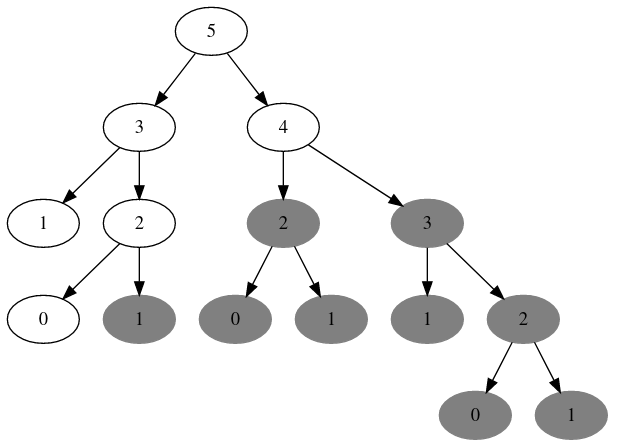
\includegraphics [scale=0.75] {fib_memo}
	\caption{Мемоизируемое вычисление $F_5$}
	\label{fig:fib_memo}
\end{figure}
\FloatBarrier

На рисунке \ref{fig:fib_memo} белым цветом обозначено непосредственное вычисление
значений $F$ с запоминанием, а серым --- получение значений из мемо-таблиц.
Вычислительная сложность на первом запуске сократилась с зачения,
сопоставимого с $O(F_n)$, до $O(n)$, тем самым приблизившись к сложности итеративного алгоритма
вычисления функции Фибоначчи. Однако мемоизируемая версия требует $O(n)$ памяти под мемо-таблицы,
когда итеративный алгоритм использует $O(1)$ памяти. В общем случае мемоизация незавершимых
или медленно сходящихся рекурсивных функций может вызвать неконтролируемую утечку памяти;
поэтому данной оптимизацией следует пользоваться с осторожностью.

\section{Обзор связанных программных средств}\label{sec:ch1/sec8}

\subsection{Enso}\label{sec:ch1/sec8/subsec1}

\textbf{Enso} --- интерактивный язык программирования с визуальным
и текстовым представлением. Enso заявлен как <<инструмент, охватывающий
весь [архитектурный] стек, начиная от высокоуровневой визуализации
и взаимодействий, и заканчивая выверенными серверными программами>> \cite{enso}.

\begin{figure}[ht]
	\centering
	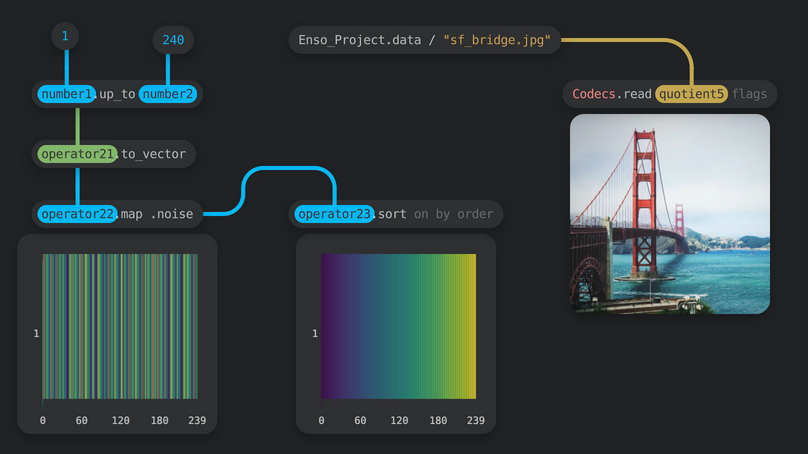
\includegraphics [scale=0.75] {enso}
	\caption{Программа на Enso}
	\label{fig:enso}
\end{figure}

\FloatBarrier

В числе особенностей Enso:

\begin{itemize}
    \item графовое визуальное представление программ;
    \item чисто функциональная семантика языка программирования;
    \item динамический (Just-in-Time) компилятор, основанный на инфраструктуре GraalVM.
\end{itemize}

В общем случае программист на Enso создает в рабочем пространстве функции
из набора примитивов стандартной библиотеки, представляемые как узлы
графовидной визуальной структуры; задает связи между функциями в виде
ребер графа, тем самым передавая значения из одной сущности языка в другую,
и параметризуя выражения.

\subsection{Adobe XD}\label{sec:ch1/sec8/subsec2}

\textbf{Adobe XD} --- это векторный инструмент проектирования пользовательского интерфейса
веб-приложений и мобильных приложений, разработанный и распространяемый Adobe Inc.
Adobe XD поддерживает создание макетов веб-сайтов и прототипов с переходом по клику \cite{adobexd}.

Имеется смысл в анализе интерфейса подобных систем с целью дальнейшего проектирования интерфейса
среды ускоренной разработки приложений и визуального программирования.

Интерфейс Adobe XD выглядит следующим образом:

\begin{figure}[ht]
	\centering
	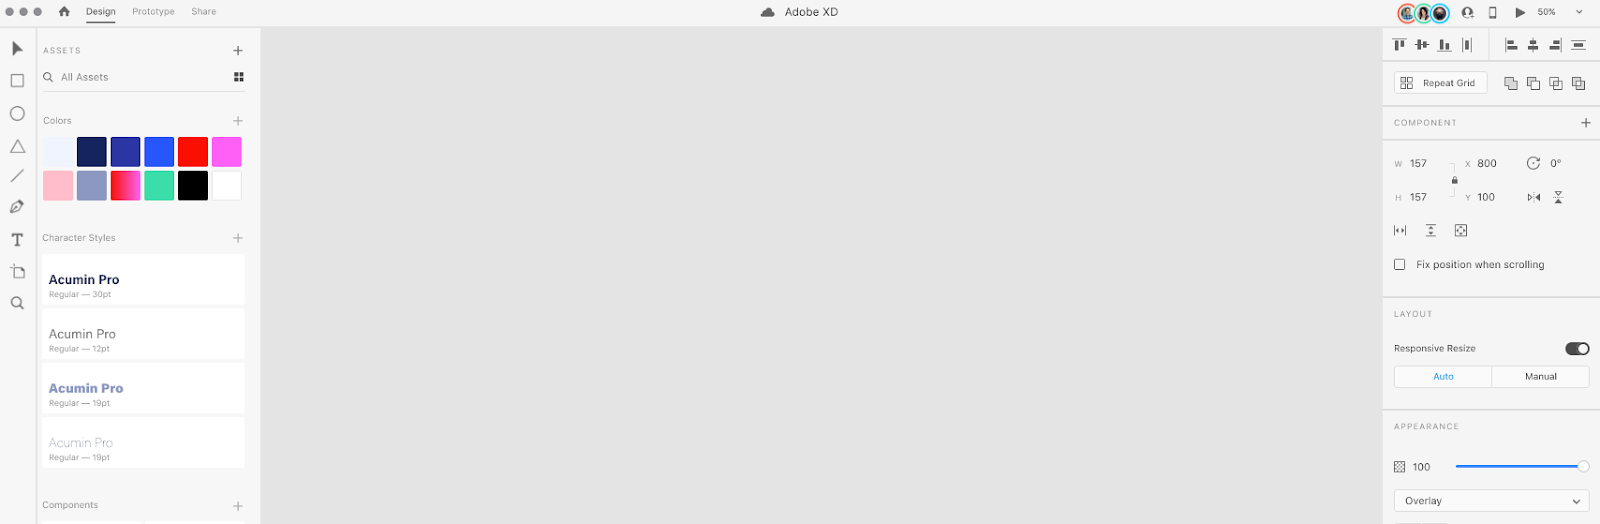
\includegraphics [scale=0.35] {adobexd}
	\caption{Интерфейс Adobe XD}
	\label{fig:adobexd}
\end{figure}

\FloatBarrier

На верхней панели расположены кнопки Design, Prototype, Share, отражающие стадии рабочей сессии
с приложением; в правой части панели расположена кнопка запуска, при нажатии на которую запускается
проектируемый прототип. Панель расположена на видном месте, содержит элементы управления для доступа
к основным окнам, содержит элемент управления, который позволяет выполнять основное,
часто повторяющееся действие --- просмотр прототипа. 
Все пользовательские действия доступны в выпадающем меню, доступ к которому открывается при нажатии
на пиктограмму типа <<стрелка вниз>>.

Главная рабочая область состоит рабочего пространства посередине, каталога компонентов в
скрываемой панели слева, настройки компонентов в панели справа.
Панели можно скрывать для удобства пользователя, тем самым максимизируя рабочую область.
Содержимое боковых панелей сгруппировано в скрываемые блоки:

\begin{figure}[ht]
	\centering
	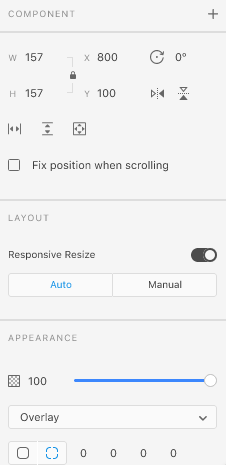
\includegraphics [scale=0.75] {adobexdblock}
	\caption{Группировка блоков на боковой панели Adobe XD}
	\label{fig:adobexdblock}
\end{figure}

\FloatBarrier

Управление содержимым рабочей области осуществляется с использованием технологии <<drag-and-drop>>.
При нажатии левой кнопкой мыши на компонент, он выделяется рамкой, его свойства отображаются в правой панели. 
При нажатии правой кнопкой мыши появляется выпадающее меню, в котором доступны функции управления компонентом.

\FloatBarrier

\subsection{Flo}\label{sec:ch1/sec8/subsec3}

\textbf{Flo} --- визуальный чисто функциональный язык программирования.
Особенности языка включают функции высшего порядка, нестрогую модель вычислений,
сильную статическую типизацию \cite{flo}.

\begin{figure}[ht]
	\centering
	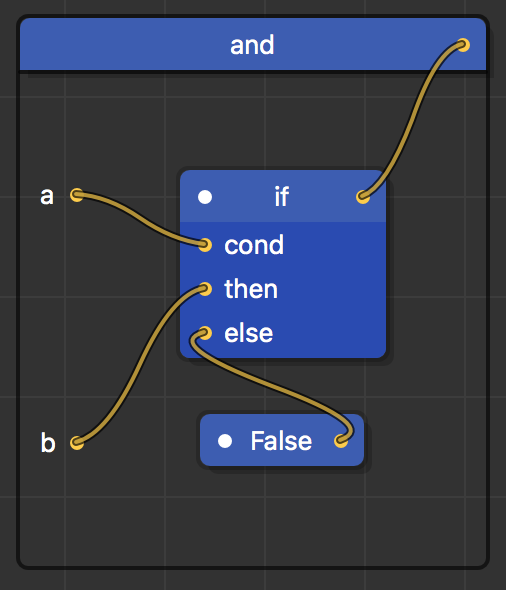
\includegraphics [scale=0.75] {flo}
	\caption{Определение функции на Flo}
	\label{fig:flo}
\end{figure}

\FloatBarrier

Основой визуального синтаксиса Flo являются <<боксы>> (англ. --- boxes), 
представляющие функции, переменные, конструкторы данных и типы. 
Боксы имеют имя, возможно пустой набор входов слева, и выход справа.

<<Кабели>> (англ. --- cables) являются второй основной составляющей
визуального синтаксиса Flo. Они используются для соединения выхода
одного бокса с входом другого, тем самым представляя поток данных.

В выражениях боксы встречаются как <<черные ящики>> с неопределенной
реализацией. Действительное содержимое боксов определяется в так
называемых <<определениях боксов>>. В качестве примера, на рисунке
\ref{fig:flo} представлено определение булевой функции <<Логическое И>>.

\section{Постановка задач на исследование}\label{sec:ch1/sec9}

В результате анализа технологий, методов, алгоритмов, была поставлена следующая цель:

\begin{itemize}
    \item проектирование и разработка интегрированной среды программирования на визуальном функциональном языке с возможностью оптимизации рекурсии.
\end{itemize}

Были выделены следующие задачи:

\begin{enumerate}
    \item проектирование визуального языка функционального программирования;
    \item проектирование и разработка интегрированной среды визуального программирования на ранее спроектированном языке;
    \item проектирование и разработка оптимизирующего компилятора программ на ранее спроектированном языке с транслятором в код на языке JavaScript в качестве целевой платформы.
\end{enumerate}

\nocite{*}

\FloatBarrier